\documentclass[10pt,times]{report}
\usepackage{url}
\usepackage{graphicx}
\setkeys{Gin}{width=\textwidth,height=\textheight,keepaspectratio}
\usepackage{caption}
\usepackage{subcaption}
\usepackage{listings}
\usepackage{xcolor}
\usepackage{framed}
\usepackage{pgfplotstable}
\usepackage{pgfplots}
\lstset{language=Python, keywordstyle=\color{blue}\bfseries, }
\usepackage{amsmath}

\setlength{\parskip}{0pt}
\setlength{\parsep}{0pt}
\setlength{\headsep}{0pt}
\setlength{\topskip}{0pt}
\setlength{\topmargin}{0pt}
\setlength{\topsep}{0pt}
\setlength{\partopsep}{0pt}

\newcommand{\lbp}{LB\_Period}

\pagestyle{myheadings}

\hyphenation{in-de-pen-dent}


\begin{document}

\begin{flushleft}
\textbf{\large{RefineLB}}
\end{flushleft}

  \begin{figure}[htbp]
    \begin{center}
       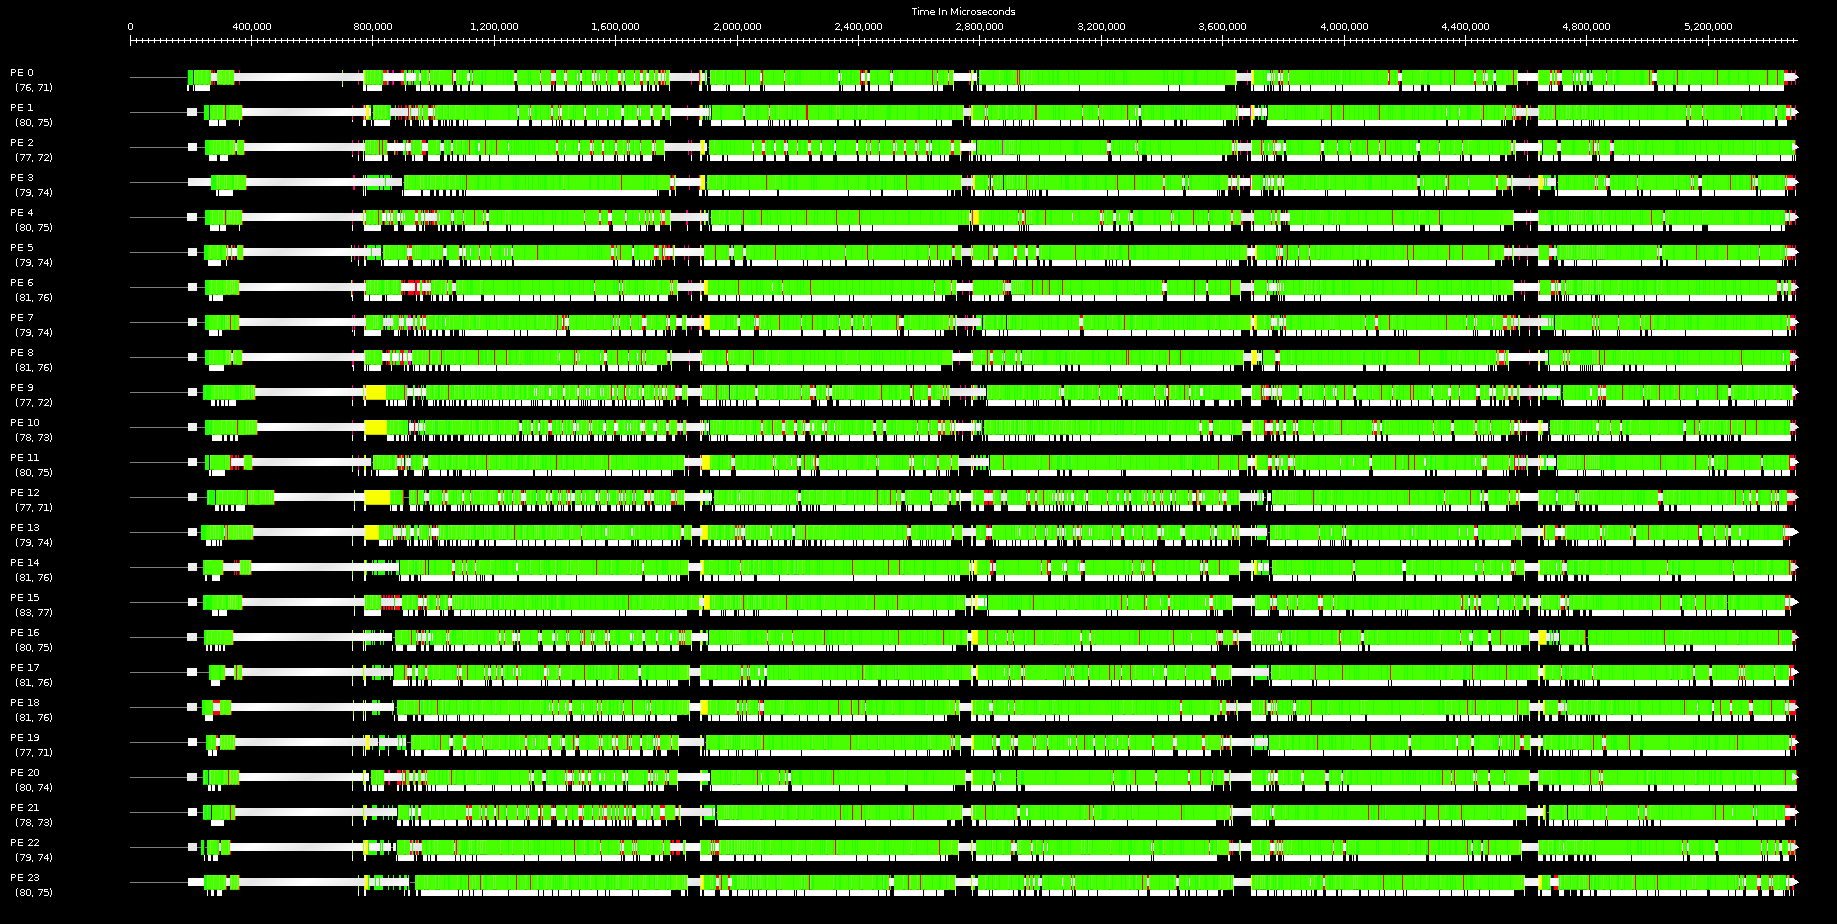
\includegraphics{TL_100_20_RLB_24.png} 
    \end{center}
    \caption{RefineLB: Cores: 24, LB\_PERIOD: 20, Iteration Count:100}
      \label{fig:1} 
  \end{figure}

  \begin{flushleft}
    \textbf{Are   they   beneficial?   Why   or   why   not?   How   much   is   the   overhead?}  
  \end{flushleft}
  Yes, they are beneficial if done less frequently. With \lbp = 10, RefineLB
  total execution time (6683 ms) is more that that of without any LB case (6070
      ms). But with \lbp = 20 we are getting better performance (RefineLB time
        = 5492 ms and NoLB time = 5955 ms). The reason is that with frequent
      load balancing the overhead of load balancing (decision time and actual
          migration time) become dominant than the actual gain obtained by load
      balancing. For example, with \lbp = 10, the load balancing overhead is
      $1.441\%$ as compared to $.860\%$ at \lbp = 20.    

  \textbf{\small{Other Overheads}}:  When we are doing RefineLB, the
  neighboring chares \textbf{MAY} get separated if they where situated  at the
  same PE during initial placement. This observation is true for any LBs
  discussed in this report ( except the GreedyComm which takes into account the
      associated communication). This also add on to communication load on CPU.

  Also the application is peculiar in two ways: \
      (1) The load is frequently changing across the chares.
      (2) With too big iteration count the application may load balance itself naturally.
    Now if we keep the iteration count be very large (e.g. with 500)
  then the RefineLB is not giving better performance (even with infrequent load balancing),  because the application is naturally balanced 
  and the load balancing effort comes as an extra overhead. 

  \begin{flushleft}
    \textbf{\small{Which  strategy  is  the  best  for  this  Particle  application?}}
  \end{flushleft}
  This strategy seems to be the best among the three discussed, with the
  constrains like LB period should not be too frequent and the iteration count
  should not be too big. The reason are: (1) The overhead of RefineLB is lower
  than others.  (2) As the load is frequently changes in the application it
  does not worth using a high overhead load balancing strategy. Rather a small
  refinement will be sufficient.

\pagebreak
\begin{flushleft}
\textbf{\Large{GreedyLB}}
\end{flushleft}

  \begin{figure}[htbp]
    \begin{center}
       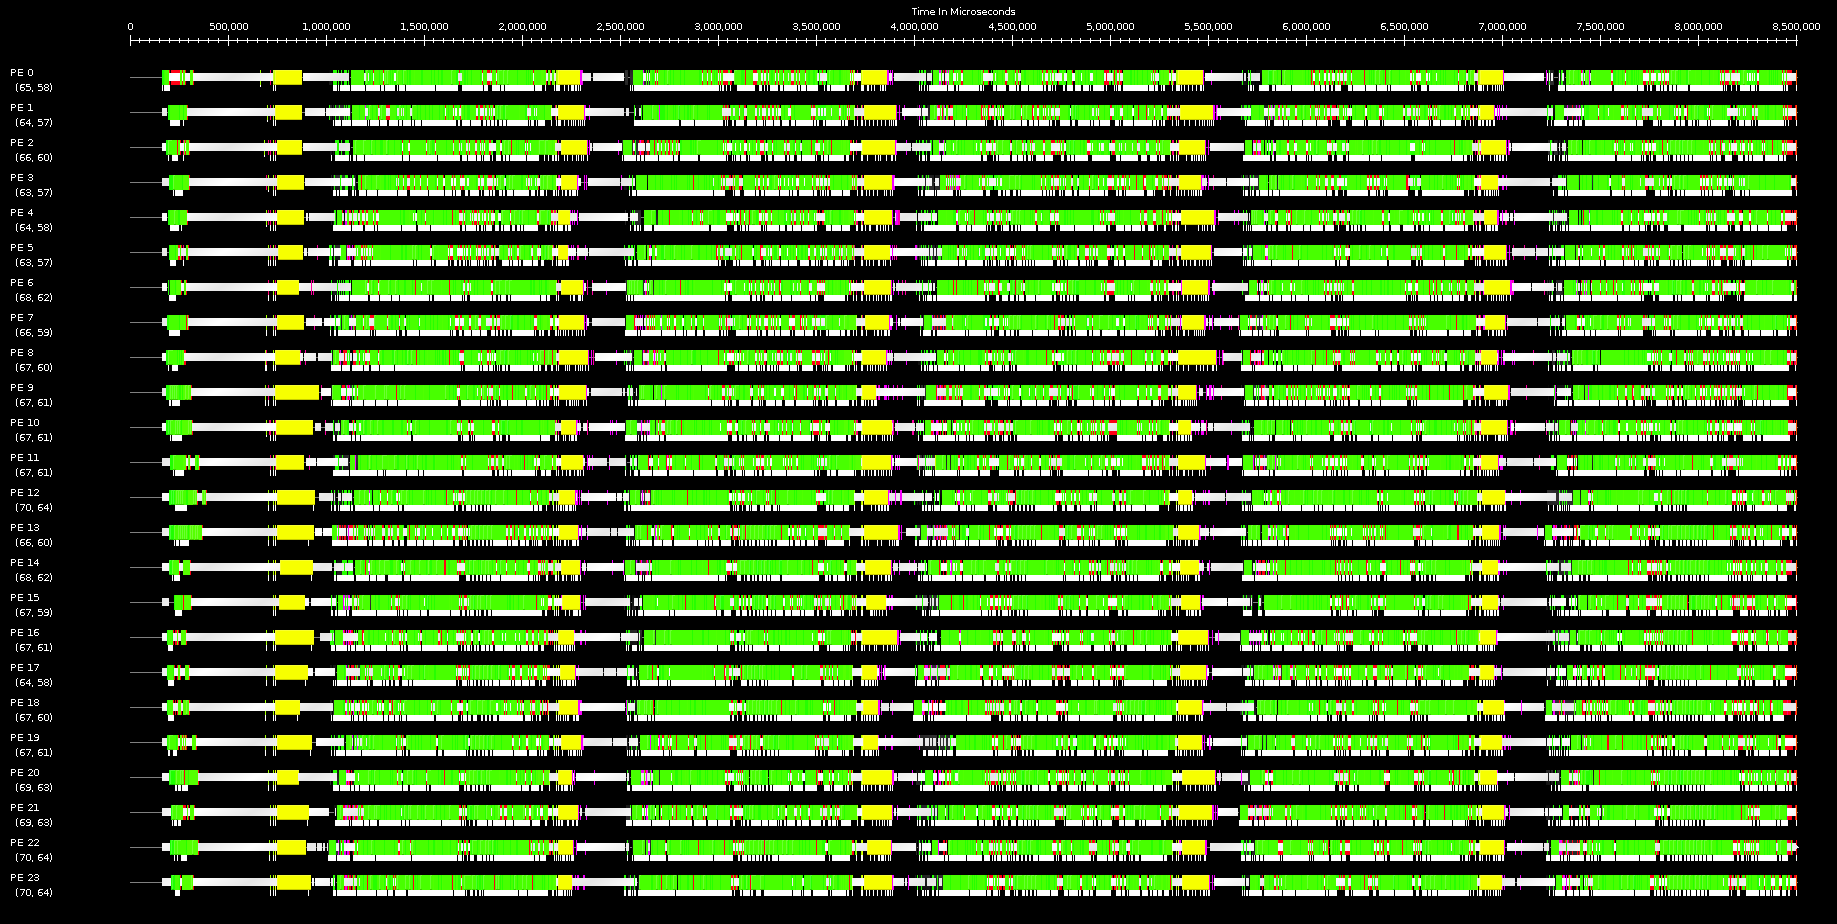
\includegraphics{TL_100_20_GLB_24.png} 
    \end{center}
    \caption{GreedyLB: Cores: 24, LB\_PERIOD: 20, Iteration Count:100}
      \label{fig:2} 
  \end{figure}

  \begin{flushleft}
    \textbf{Are   they   beneficial?   Why   or   why   not?   How   much   is   the   overhead?}  
  \end{flushleft}
  NOT beneficial. The following table with different \lbp\ values shows that GreedyLB's total execution times are  more than those with NoLB and RefineLB.

  \begin{table}[h]
  \begin{tabular}{|c|c|c|c|c|c|}
  \hline
  \multicolumn{1}{|l|}{LB\_Period} & \multicolumn{1}{l|}{$t_{nolb} (ms)$} &
  \multicolumn{1}{l|}{$t_{rlb} (ms) ( \% p_{rlb})$} &
  \multicolumn{1}{l|}{$t_{glb} (ms) (\%p_{glb})$} \\ \hline 10
  &  6070                     & 6683   (1.441)                   & 9830  (11.5)
  \\ \hline 20                           &  5955                     & 5492
  (.860)                    & 8503  (7.112)                           \\ \hline
  30                           &  5876                     & 5277   (.60)
  & 5989  (5.51)                        \\ \hline \end{tabular} \caption
{$t_{nolb},\ t_{rlb},\ t_{glb}$ are the application execution times with NoLB, RefineLB and
  GreedyLB respectively and $p_{rlb},\ p_{glb}$ are the \% CPU utilization for
    the migrations.} \end{table}
 
The reason is that the overhead of GreedyLB load balancing  (decision time and
    actual migration time) is very high. Though the quality of load balancing
provided by GreedyLB is much better than RefineLB, but that does not help in
this scenario because (1) The load is frequently changing across the chares. So
the effort put in by this expensive load balancing is kind of nullified after
few iterations.  (2) In case of GreedyLB, the number of chares migrated in more
as compared to RefineLB and that migration happens without taking communication
into account, so this ends up with decoupling the neighboring chares which in
turn causes huge communication load on CPU.

\underline{Another interesting observation} is as the \lbp\ decreases, the overhead of load
balancing diminishes and so the total execution time.      Also with higher
iteration count, the performance is bad as compared to both NoLB and RefineLB
because the application get naturally load balanced in that scenario and the
effort of this expensive load balancing becomes an overhead.

\pagebreak

\begin{flushleft}
\textbf{\Large{GreedyCommPB}}
\end{flushleft}

  \begin{figure}[htbp]
    \begin{center}
       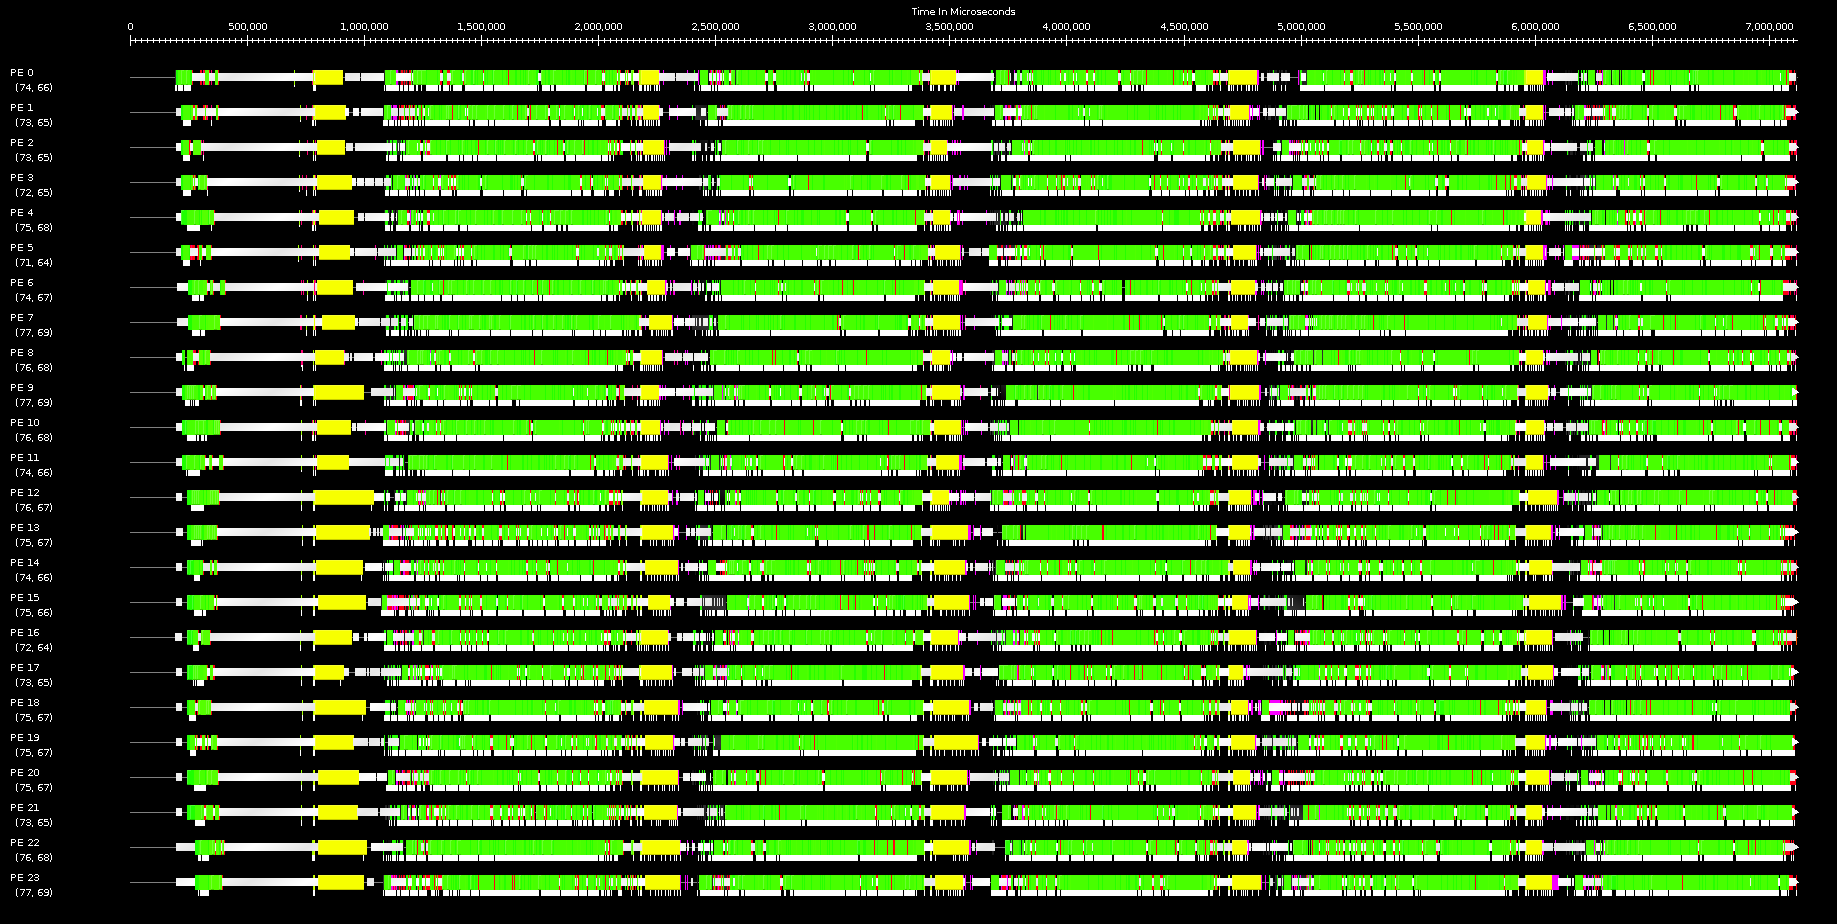
\includegraphics{TL_100_20_GCLB_24.png} 
    \end{center}
    \caption{GreedyLB: Cores: 24, LB\_PERIOD: 20, Iteration Count:100}
      \label{fig:3} 
  \end{figure}

  \begin{flushleft}
    \textbf{Are   they   beneficial?   Why   or   why   not?   How   much   is   the   overhead?}  
  \end{flushleft}
  NOT beneficial. The following table with different \lbp\ values shows that
  GreedyCommLB's total execution times are  more than those with NoLB and
  RefineLB.  The reason for this is same as the reasons for GreedyLB that the
  overhead of migration is huge which is not beneficial in the scenario when
  the load is dynamically changing. Also similar to GreedyLB they end up
  decoupling the neighboring chares adding more to the communication load of
  CPU.
  
  \text{BUT} there performance is better than GreedyLB because they are
  communication aware in the sense that if two chares are going to communicate
  much then they will be kept on the same PE.

  \begin{table}[h]
  \begin{tabular}{|c|c|c|c|c|c|}
  \hline
  \multicolumn{1}{|l|}{LB\_Period} & \multicolumn{1}{l|}{$t_{nolb} (ms)$} &
  \multicolumn{1}{l|}{$t_{rlb} (ms) ( \% p_{rlb})$} &
  \multicolumn{1}{l|}{$t_{glb} (ms) (\%p_{glb})$} &
  \multicolumn{1}{l|}{$t_{gclb} (ms) (\%p_{gclb})$}\\ \hline 10
  &  6070                     & 6683   (1.441)                   & 9830  (11.5)
  &    9817 (12.56)     \\ \hline 20                           &  5955
  & 5492   (.860)                    & 8503  (7.112)               &    7117
  (8.04)         \\ \hline 30                           &  5876
  & 5277   (.60)                     & 5989  (5.51)                &    5914
  (4.54)         \\ \hline \end{tabular} \caption {The application is run on 24
    cores with iteration Count 100.  $t_{nolb},\ t_{rlb},\ t_{glb}\ and\
      t_{gclb}$ are the executions times of NoLB, RefineLB, GreedyLB and
      GreedyCommLB respectively and $p_{rlb},\ p_{glb}\ and\ p_{gclb}$ are the
      \% CPU utilization for the migrations of RefineLB, GreedyLB and
      GreedyCommLB respectively.} \end{table}

Also like GreedyLB, as the \lbp\ decreases, the overhead of load balancing
diminishes and so the total execution time.  Also with higher iteration count,
           the performance is bad as compared to both NoLB and RefineLB,
           \textbf{BUT} better that GreedyLB.

  
\end{document}

% \usepackage{multirow}
%\begin{table}[h]
%\begin{tabular}{|l|c|c|c|c|c|c|}
%\hline
%Total Iteration      & \multicolumn{1}{l|}{Period} & \multicolumn{1}{l|}{Cores} & \multicolumn{1}{l|}{WLB} & \multicolumn{1}{l|}{RLB (Overhead)} & \multicolumn{1}{l|}{GLB} & \multicolumn{1}{l|}{GCLB} \\ \hline
%\multirow{6}{*}{100} & 10                          & 12                         & 9563                     & 10005 (1.083)                       & 12688(15.68)             & 12124 (15.07))            \\ \cline{2-7} 
%                     &                             & 24                         & 6070                     & 6683(1.441)                         & 9830 (11.5)              & 9877 (12.56)              \\ \cline{2-7} 
%                     & 20                          & 12                         & 9094                     & 9063 (.486)                         & 10690 (9.4)              & 10580 (9.331)             \\ \cline{2-7} 
%                     &                             & 24                         & 5955                     & 5492 (.860)                         & 8503 (7.112)             & 7117 (8.04)               \\ \cline{2-7} 
%                     & 50                          & 12                         & 8988                     & 9151 (.44)                          & 9550 (4.24))             & 9413 ( 4.91)              \\ \cline{2-7} 
%                     &                             & 24                         & 5876                     & 5277 (.60)                          & 5989 (5.51)              & 5914 (4.54)               \\ \hline
%\multirow{6}{*}{500} & 10                          & 12                         & 9527                     & 10220                               & 12671                    & 12435                     \\ \cline{2-7} 
%                     &                             & 24                         & 6510                     & 11194                               & 12801                    & 9730                      \\ \cline{2-7} 
%                     & 20                          & 12                         & 9026                     & 9468                                & 10311                    & 10242                     \\ \cline{2-7} 
%                     &                             & 24                         & 6090                     & 8634                                & 9439                     & 7393                      \\ \cline{2-7} 
%                     & 50                          & 12                         & 8957                     & 9221                                & 9975                     & 9548                      \\ \cline{2-7} 
%                     &                             & 24                         & 5762                     & 7784                                & 6230                     & 7485                      \\ \hline
%\end{tabular}
%\end{table}
